\documentclass[letterpaper]{article}

% Core packages
\usepackage[top=1in,bottom=1in,left=1in,right=1in]{geometry}
\usepackage{graphicx}
\usepackage{multicol}
\usepackage{fancyhdr}
\usepackage{eso-pic}
\usepackage[explicit]{titlesec}
\usepackage{varwidth}
\usepackage{parskip}
\usepackage{tgcursor}
\usepackage{fontspec}

% Font setup
\fontsize{10pt}{10pt}\selectfont
\setmainfont[
  Path=fonts/,
  Extension=.ttf
]{Typewriter-Executive}

% Graphics paths
\graphicspath{{pages/}}

% Page number settings
\pagestyle{fancy}
\fancyhf{}                    % Clear all headers and footers
\fancyfoot[C]{-\thepage-}     % Bottom center: -1-
\renewcommand{\headrulewidth}{0pt}
\renewcommand{\footrulewidth}{0pt}
\setlength{\footskip}{24pt}

% Body text settings
\parskip=8pt
\parindent=3em
\setcounter{secnumdepth}{0}
\setlength{\fboxsep}{6pt}

% Section styling
\titleformat{\section}[block]
  {\normalfont\large\bfseries\centering}
  {}
  {0pt}
  {\makebox[\linewidth][c]{\fbox{\begin{varwidth}{\linewidth}\centering #1\end{varwidth}}}}
\titlespacing*{\section}{0pt}{*2}{*1}
%%%%%%%%%%%%%%%%%%%%%%%%%%%%%%%%%%%%%%%%%%%%%
\begin{document}
\begin{titlepage}
\thispagestyle{empty}
\centering


\includegraphics[width=0.5\textwidth]{logo.png}\vspace{2.5cm}

{\bf \Huge
APPLE-1
\vspace{1cm}

OPERATION

MANUAL
}
\vspace{2cm}

{\fontspec{Helvetica}
APPLE COMPUTER COMPANY

770 Welch Road

Palo Alto, California 94304
}
\end{titlepage}
%%%%%%%%%%%%%%%%%%%%%%%%%%%%%%%%%%%%%%%%%%%%%
\begin{center}
  SPECIFICATIONS
\end{center}
\begin{tabular}{p{0.46\textwidth} p{0.46\textwidth}}
  
MICROPROCESSOR:&MOS Technology 6502\\

Microprocessor Clock Frequency:&1.023 MHz\\

Effective Cycle Frequency:&0.960 Mhz\\

(Including Refresh Waits)&\\

VIDEO OUTPUT:&Composite positive video, 75 ohms, level adjustable between zero and +5V pp.\\

Line Rate:&15734 Hz\\
Frame Rate:&60.06 Hz\\
Format&40 characters/line, 24 lines; with automatic scrolling\\
Display Memory:&Dynamic shift registers (1K x 7)\\
Character Matrix:&5 x 7\\
\end{tabular}
\clearpage
\setcounter{page}{1}
\newpage
\begin{center}
\section{INTRODUCTION}
\end{center}
\begin{multicols}{2}

The Apple Computer is a complete microprocessor system, consisting of a Mos Technology 6502 microprocessor and support hardware, integral video display electronics, dynamic memory and refresh hardware, and fully regulated power supplies. It contains resident system monitor software, enabling the user, via the keyboard and display, to write, examine, debug, and run programs efficiently; thus being an educational tool for the learning of microprocessor programming, and an aid in the development of software.


The integral video display section and the keyboard interface renders unnecessary the need for an external teletype. The display section contains its ownmemory, leaving all of RAM for user programs, and the output format is 40 characters/ line, 24 lines/page, with auto scrolling. Almost any ASCII encoded keyboard will interface directly with the Apple system.

The board has sockets for upto 8K bytes of the 16 pin, 4K type, RAM, and the system is fully expandable to 65K via the edge connector. The system uses dynamic memory (4K bytes supplied), although static memory may also be used. All refreshing of dynamic memory, including all "off-board'" expansion memory, is done automatically. The entire system timing, including the microprocessor clock and all video signals, originates in a single crystal oscillator.

Further, the printed circuit board contains a "breadboard area", in which the user can add additional "on-board" hardware (for example, extra PIA's, ACIA's, EROM's, and so on).

This manual is divided into three Sections:

\noindent Section I GETTING THE SYSTEM RUNNING

\noindent Section II USING THE SYSTEM MONITOR. (listing included)

\noindent Section III EXPANDING THE SYSTEM.

Please read Section I thoroughly, before attempting to "power-up" your system, and study Section III carefully before attempting to expand your system. In addition to this manual, Apple 'Tech Notes" are available which contain examples of expansion hardware and techniques.
\end{multicols}
\begin{center}
\section{SECTION I
\newline
GETTING THE SYSTEM RUNNING}   
\end{center}


\begin{multicols}{2}
The Apple Computer is fully assembled, tested, and burned in. The only external devices necessary for operation of the system are: An ASCII encoded keyboard, a video display monitor, and AC power sources of 8 to 10 Volts (RMS) @3 amps and 28Volts(RMS)@1 amp. The following three articles describe the attachment of these devices in detail.

\noindent Keyboard:

Any ASCII encoded keyboard, with positive DATA outputs, interfaces directly with the Apple system via a "DIP" connector, If your keyboard has negative logic DATA outputs (rare), you can install inverters (7404) in the breadboard area. The strobe can be either positive or negative, of long or short duration. The 'DIP" keyboard connector (B4) has inputs for seven DATA lines, one STROBE line, and two normally-open pushbutton switches, used for RESET (enter monitor), and CLEAR SCREEN (see schematic diagram, sheet 3 of 3, for exact circuitry). This keyboard connector also supplies three voltages, (45V, +12V, and-12V) of which one or more may be necessary to operate the keyboard. Pin 15 of the keyboard connector (B4) must be tied to +5V (pin 16) for normal operation,

\noindent NOTE: The system monitor accepts only uppercase alpha (A-F, R).

It is therefore convenient, though it's not essential, to have akeyboard equipped with uppercase alpha lock (usually in the electronics). Either of the following suggested circuits may be used to provide alpha lock capability, if needed, and can be built in the breadboard area.
\AddToShipoutPictureBG*{
  \AtPageLowerLeft{
    \makebox[\paperwidth][c]{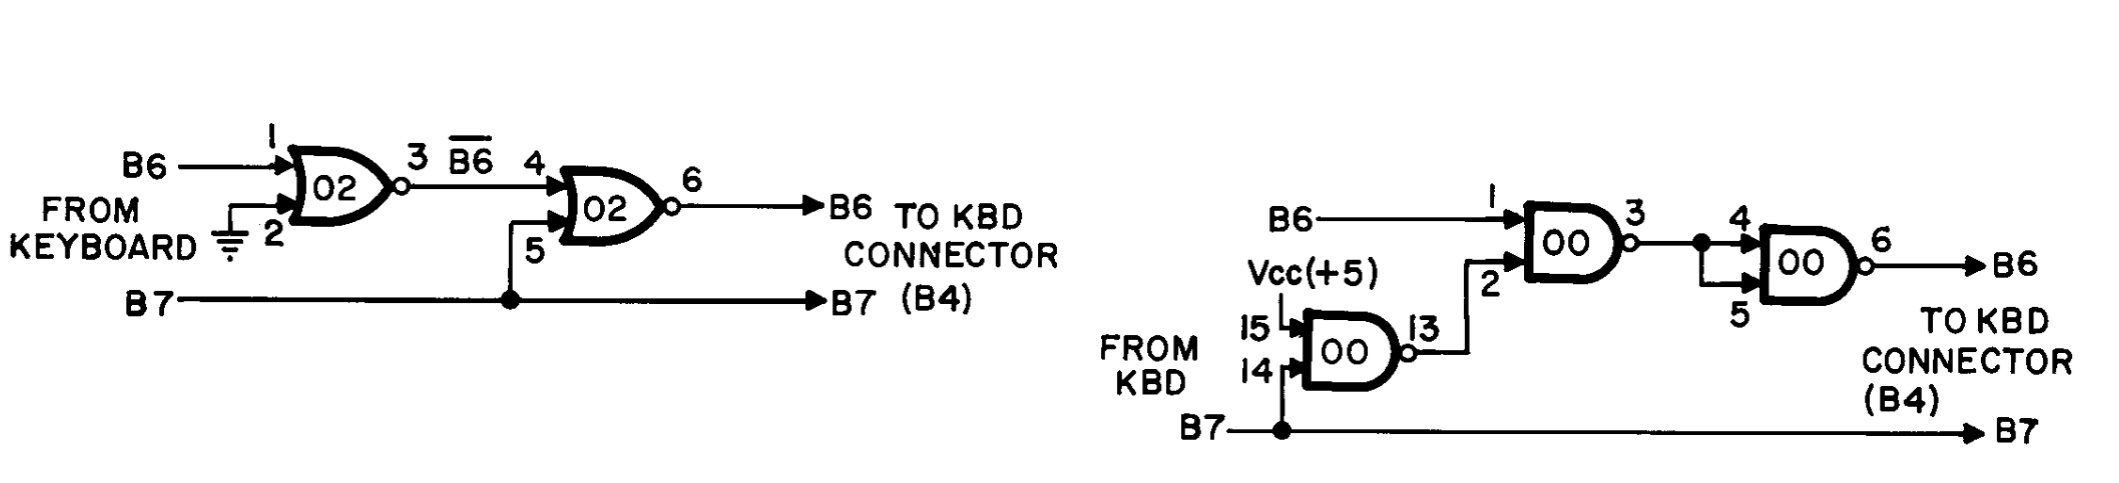
\includegraphics[width=\paperwidth]{p1_kb.png}}%
  }
}



\newpage
\noindent Display:

The Apple Computer outputs a composite video signal (composite of sync and video information) which can be applied to any standard raster-scan type video display monitor. The output level is adjustable with the potentiometer located near the video output Molex connector, J2. The additional two outside pins on the Molex connector supply +5and+l2 volts, to be used in future Apple accessories. The composite video signal can also be modulated atthe proper RF frequency, with an inexpensive commercially available device, and applied to the antenna terminals of a home television receiver. Since the character format is 40 characters /line, all television receivers will have the necessary bandwidth to display the entire 40 characters. Two large manufacturers of video display monitors, which connect directly with the Apple Computer, are Motorola and Ball. The mating four-pin Molex connector is provided.

\noindent AC Power Sources:

Two incoming AC power sources are required for operation: 8tol0 VAC (RMS) at 3 amps, and 28VAC(RMS) Center-Tapped at lamp. These AC supplies enter the system at the Molex connector, Jil. The 8tol0 volts AC provides the raw AC for the +5 volt supply, while the 28 VCT supplies the raw AC for the +12 and -12 volt supplies, and the -5V supply is derived from the -12V regulated output.

The board, as supplied, requires no more than 1.5 amps DC from the 45V supply, while the regulator is capable of supplying 3 amps. The remaining 1.5 amps DC from the 45V supply is available for user hardware expansion (provided suitable transformer ratings are employed).

A suitable source of the raw AC voltages required, are two commercially available trans— formers; Stancor P/N P-8380 or equivalent (8 to 10 volts at 3 amps), and Stancor P/N P-8667 or

equivalent (28VCT at 1 amp). Simply wire the secondaries tothe mating six~pin Molex connector supplied, and wire the primaries in parallel, as shown in the schematic diagram (power supply section, Dwg.No. 00101, sheet 3 of 3.

\noindent TEST PROGRAM

After attaching the keyboard, display, and AC power sources, you can try a simple program to test if your system and the attachments are functioning together properly. While it does not test many possible areas of the microprocessor system, the test program will test for the correct attachment of the keyboard, display, and power supplies.

FIRST:

Hit the RESET button to enter the system monitor. A backslash shouldbe displayed, andthecursor shoulddroptothe nextline,

SECOND:

Type- $\emptyset$:A9b$\emptyset$ bAAK2$\emptyset$bEFbDFF bd E8 b 8A b4C b2b$\emptyset$ (RET)

($\emptyset$ is a zero, NOT an alpha "''"O''; b means blank or space; and (RET) hit the ''return!" key on the keyboard)

THIRD:

Type- $\emptyset$.A(RET)

(This should print out, on the display, the program you have just entered,)

FOURTH: Type- R(RET) (R means run the program.)

THE PROGRAM SHOULD THEN PRINT OUT ON THE DISPLAY A CONTINUOUS STREAM OF ASCII CHARACTERS, TO STOP THE PROGRAM AND RETURNTOTHE SYSTEM MONITOR, HIT THE "RESET" BUTTON. TO RUN AGAIN, TYPE: R (RET).
\end{multicols}
\newpage
\begin{center}
\section{SECTION II
USING THE SYSTEM MONITOR}
\end{center}
\begin{multicols}{2}
The Hex Monitor is a PROM program in locations FF$\emptyset$$\emptyset$ to FFFF (hex) which uses the keyboardand display to perform the front panel functions of examining memory, and running programs. The monitor program is entered by hitting (RESET), which displays backslash-return. A backslash alone (cursor remains on same line as backslash) indicates bad page 0 RAM.

Commands are typed on a "line-at-a-time" basis with editing. Each line may consist of any number of commands (up to l28 characters). None are executed until (RETURN) is typed. The (SHIFT-0) (backarrow) backspaces and echos an underline. The (ESC) cnacels a line and echos backslash-return.

One or more hexadecimal digits (0-9, A-F) are used for address and data values. Addresses use the four least significant digits of a group, and data values, the two least significant digits. The following examples illustrate the variety of acceptable commands:
\begin{enumerate}
\item Opening a location (examining the contents of a single address).

USER TYPES/ 4F (RET)

MONITOR TYPES/ $\emptyset$$\emptyset$4F: $\emptyset$F (contents of 4F)

\item Examining a block; fromthe last examined location, to a specified one.

USER TYPES/ .5A (RET)

MONITOR TYPES/ $\emptyset$$\emptyset$5$\emptyset$: $\emptyset$$\emptyset$ $\emptyset$1 $\emptyset$2 $\emptyset$3 $\emptyset$4 $\emptyset$5 $\emptyset$6 $\emptyset$7 $\emptyset$$\emptyset$58: $\emptyset$8 $\emptyset$9 $\emptyset$A 

Note: 4F is still considered the most recently opened location.

\item Combining examples 1 and 2 to print a block of memory in a single command.

USER TYPES/ 4F,5A (RET)

MONITOR TYPES  $\emptyset$$\emptyset$5$\emptyset$: $\emptyset$$\emptyset$ $\emptyset$1 $\emptyset$2 $\emptyset$3 $\emptyset$4 $\emptyset$5 $\emptyset$6 $\emptyset$7 $\emptyset$$\emptyset$58: $\emptyset$8 $\emptyset$9 $\emptyset$A 

Note: Only the first location of the block (4F) is considered "opened!".

\item Examining several individual locations at once.

USER TYPES/ AF b 52 b 56 (RET)

MONITOR TYPES/ $\emptyset$$\emptyset$4F: $\emptyset$F $\emptyset$$\emptyset$52: $\emptyset$2 $\emptyset$$\emptyset$56: $\emptyset$6

Note:

56 is considered the most recently "opened" location. The 'b' is a blank or comma, and is a delimiter for separation purposes only. A string of delimiters has the same effect as a single one (bbb is as effective as b).

\item Examining several blocks of memory at once.

USER TYPES/ 4F. 52 b 56 b 58.5A (RET)

MONITOR TYPES/ $\emptyset$$\emptyset$4F: $\emptyset$F

$\emptyset$$\emptyset$52: $\emptyset$2

$\emptyset$$\emptyset$56: $\emptyset$6

$\emptyset$$\emptyset$58: $\emptyset$8 $\emptyset$9 $\emptyset$5A: $\emptyset$A


Note: 58is considered the most recently opened” location. Refer to example 2.

\item Examining successive blocks.

USER TYPES/ 4F.52 (RET)

MONITOR TYPES/ $\emptyset$$\emptyset$4F: $\emptyset$F $\emptyset$$\emptyset$5$\emptyset$: $\emptyset$$\emptyset$ $\emptyset$1 $\emptyset$2

USER TYPES/ .55 (RET)

MONITOR TYPES/ $\emptyset$$\emptyset$53: $\emptyset$3 $\emptyset$4 $\emptyset$5

USER TYPES/ .5A (RET)

MONITOR TYPES/ $\emptyset$$\emptyset$56: $\emptyset$6 $\emptyset$7

$\emptyset$$\emptyset$58: $\emptyset$8 $\emptyset$9 $\emptyset$A

\item Depositing data in a single location.

USER TYPES/ 3$\emptyset$: A$\emptyset$ (RET)

MONITOR TYPES/ $\emptyset$$\emptyset$3$\emptyset$: FF (prior contents)

Location 39 is considered opened and now contains 39.

\item Depositing data in successive locations from that last used in a deposit command.

USER TYPES/ : Al b A2 b A3 b A4

b A5 (RET)

(This deposits Al in location 31, A2 in 32, and so on.)

\item Combining examples 7 and 8 in a single command.

USER TYPES/ 3$\emptyset$: A$\emptyset$ b Al b A2 b

A3 b A4 b A5 (RET)

MONITOR TYPES/

$\emptyset$$\emptyset$3$\emptyset$: FF (prior contents of location 3$\emptyset$)

\item Depositing data in successive locations with separate commands.

USER TYPES/ 3$\emptyset$: A$\emptyset$ b A1 (RET)
MONITOR TYPES/ $\emptyset$$\emptyset$3$\emptyset$: FF
USER TYPES/ :A2 b A3 (RET)
USER TYPES/ :A4 b A5 (RET)
\newpage

Note: A colon in a command means "start depositing data from the most recently deposited location, or if none, then from the most recently opened one.

\item Examining a block, then depositing into it. 

USER TYPES/ 30.35 (RET)

MONITOR TYPES/ 

$\emptyset$$\emptyset$3$\emptyset$: A$\emptyset$ Al A2 A3 A4 A5 A6

USER TYPES/

:B0 b B1 b B2 b B3 b B4 b B5 (RET)

Note: New data deposited beginning at most recently opened location (39)

\item Run a program at a specified address.

USER TYPES/ 1$\emptyset$F$\emptyset$ R (RET)

MONITOR TYPES/ 1$\emptyset$F$\emptyset$: A9 (contents)

Note: The cursor is left immediately to the right of the 'A9"'; it is not returned to the next line.

\item Run atthe most recently examined location.

USER TYPES/ 1$\emptyset$F$\emptyset$ (RET)

MONITOR TYPES/ 1$\emptyset$F$\emptyset$: A9

USER TYPES/ R (RET)

\item Enter a program into memory and run it in one line.

USER TYPES/ 4$\emptyset$: A9 b $\emptyset$ b 2$\emptyset$ b EF b FF b 38 b 69 b

MONITOR TYPES/ 4$\emptyset$: FF (prior contents of 4$\emptyset$)
MONITOR TYPES/ 4$\emptyset$: FF (prior contents of 4$\emptyset$)

\item An "on line" error correction.

USER TYPES/

4$\emptyset$: Al b A2 b A3A4A5\underline{A6} b A7

 (data A6 will be loaded in location 42)
 
 USER TYPES/ 4$\emptyset$5$\emptyset$6$\emptyset$7$\emptyset$: AA

 (data AA will be loaded in location 6$\emptyset$7$\emptyset$)

 \item Useful routines in monitor which can be accessed by user programs.
 
 GETLINE: location FF1F:
 
 monitor entry point

(jumping to FF1F will enter monitor and echo carriage return. You can then examine memory locations with the monitor.)

ECHO: location FFEF:

prints one byte (ASCII)

(data from "A" (accumulator), contents of ''A'' not disturbed. Example:

2$\emptyset$ b EF b FF (JRS ECHO)).

PRBYTE: location FFDC:

prints one byte (HEX)

(data from "A", contents of "A" disturbed.) 

PRHEX: location FFES5:

rints one hex digit

(data from four least significant bits of "A", contents of "A" disturbed.)
\end{enumerate}
\end{multicols}
\begin{center}
NOTE: Capital letters enclosed in parenthesis represent single keystrokes.
Example: (RET) means hit the "return" key
\end{center}
\newpage
\begin{multicols}{2}

\end{multicols}
\begin{center}
NOTE: RAM locations $\emptyset$$\emptyset$24 to $\emptyset$$\emptyset$2B are used as index pointers by the monitor, and are invalid for user use, when using monitor. Also, locations $\emptyset$$\emptyset$2$\emptyset$ to $\emptyset$27F are used as input buffer storage, and are also invalid for user use when using the monitor.

\newpage

65$\emptyset$2 HEX MONITOR LISTING
\end{center}

\begin{tabbing}
FF$\emptyset\emptyset$\hspace{.18in}\=D8\hspace{.75in}\=RESET\hspace{.5in}\=CLD\hspace{1.25in}\={\rmfamily Clear Decimal arithmetic mode}\\
FF$\emptyset$1\>58\>\>CLI\>\\
FF$\emptyset$2\>A$\emptyset$ 7F\>\>LDY \#\$7F\>{\rmfamily Mask for DSP data direction register}\\
FF$\emptyset$4\>8C 12 D$\emptyset$ \> \>STY DSP \>{\rmfamily Set it up}\\
FF$\emptyset$7\>A9 A7\>\>LDA \#\$A7\>{\rmfamily KBD and DSP control register mask}\\
FF$\emptyset$9\>8D 11 D$\emptyset$\>\>STA KBD CR\>{\rmfamily Enable interrupts, set CA1, CB1, for}\\
FF$\emptyset$C\>8D 11 D$\emptyset$\>\>STA DSP CR\> {\rmfamily \hspace{.125in}positive edge sense/output mode}\\
FF$\emptyset$F\>8D 13 D$\emptyset$\>NOTOR\>CMP \#\$DF\>{\rmfamily "$\Leftarrow$"?}\\
FF11\>F$\emptyset$ 13\>\>BEQ BACKSPACE\>{\rmfamily Yes.}\\
FF13\>C9 9B\>\>CMP \#\$9B\>{\rmfamily ESC?}\\
FF15\>F$\emptyset$ 03\>\>BEQ ESCAPE\>{\rmfamily Yes.}\\
FF17\>C8\>\>INY\>{\rmfamily Advance text index.}\\
FF18\>1$\emptyset$ $\emptyset$F\>\>BPL NEXTCHAR\>{\rmfamily Auto ESC if > 127.}\\
FF1A\>A9 DC\>ESCAPE\>LDA \#\$DC\>{\rmfamily "$\backslash$".}\\
FF1C\>20 EF FF\>\>JSR ECHO\>{\rmfamily Output it.}\\
FF1F\>A9 8D\>GETLINE\>LDY \#\$$\emptyset$1\>{\rmfamily CR.}\\
FF21\>2$\emptyset$ EF FF\>\>JSR ECHO\>{\rmfamily Output it.}\\
FF24\>A$\emptyset$ $\emptyset$1\>\>LDY \#\$$\emptyset$1\>{\rmfamily Initialize text index.}\\
FF26\>88\>BACKSPACE\>DEY\>{\rmfamily Back up text index.}\\
FF27\>3$\emptyset$ F6\>\>BMI GETLINE\>{\rmfamily Beyond start of line, reinitialize.}\\
FF29\>AD 11 D$\emptyset$\>NEXTCHAR\>LDA KBD CR\>{\rmfamily Key ready?}\\
FF2C\>1$\emptyset$ FB\>\>BPL NEXTCHAR\>{\rmfamily Loop until ready.}\\
FF2E\>AD 1$\emptyset$ D$\emptyset$\>\>LDA KBD\>{\rmfamily Load Character. B7 should be '1'.}\\
FF31\>99 $\emptyset$$\emptyset$ $\emptyset$2\>\>STA IN, Y\>{\rmfamily Add to text buffer.}\\
FF34\>2$\emptyset$ EF FF\>\>JSR ECHO\>{\rmfamily Display character.}\\
FF37\>C9 8D\>\>CMP \#\$8D\>{\rmfamily CR?}\\
FF39\>D$\emptyset$ D4\>\>BNE NOTOR\>{\rmfamily No.}\\
FF3B\>A$\emptyset$ FF\>\>LDY \#\$FF\>{\rmfamily Reset text index.}\\
FF3D\>A$\emptyset$ FF\>\>LDA \#\$$\emptyset\emptyset$\>{\rmfamily For XAM mode.}\\
FF3F\>AA\>\>TAX\>{\rmfamily $\emptyset\rightarrow$ X}\\
FR4$\emptyset$\>$\emptyset$A\>SETSTOR\>ASL\>{\rmfamily Leaves \$7B if setting STOR mode.}\\
FF41\>85 2B\>SETMODE\>STA MODE\>{\rmfamily \$$\emptyset\emptyset$ = XAM, \$7B = STOR, \$AE = BLOK XAM.}\\
FF43\>C8\>BLSKIP\>INY\>{\rmfamily Advance text index.}\\
FR44\>B9 $\emptyset$$\emptyset$ $\emptyset$2\>NEXT ITEM\>LDA IN, Y\>{\rmfamily Get character.}\\
FF47\>C9 8D\>\>CMP \#\$8D\>{\rmfamily CR?}\\
FF49\>F$\emptyset$ D\>\>BEQ GETLINE\>{\rmfamily Yes, done this line.}\\
FF4B\>C9 AE\>\>CMP \#\$AE\>{\rmfamily "."?}\\
FF4D\>9$\emptyset$ F4\>\>BCC BLSKIP\>{\rmfamily Skip delimiter.}\\
FF4F\>F$\emptyset$ F$\emptyset$\>\>BEQ SETMODE\>{\rmfamily Set BLOCK XAM mode.}\\
FF51\>C9 BA\>\>CMP \#\$BA\>{\rmfamily ":"?}\\
FF53\>F$\emptyset$ EB\>\>BEQ SETSTOR\>{\rmfamily Yes, set STOR mode.}\\
FF55\>C9 D2\>\>CMP \#\$D2\>{\rmfamily "R"?}\\
FF57\>F$\emptyset$ 3B\>\>BEQ RUN\>{\rmfamily Yes, run user program.}\\
FF59\>86 28\>\>STX L\>{\rmfamily \$$\emptyset\emptyset\rightarrow$L.}\\
FF5B\>86 29\>\>STX H\>{\rmfamily \hspace{.125in}and H.}\\
FF5D\>84 2A\>\>STY YSAV\>{\rmfamily Save Y for comparison.}\\
FF5F\>B9 $\emptyset\emptyset$ $\emptyset$2\>NEXTHEX\>LDA IN, Y\>{\rmfamily Get character for hex test.}\\
FF62\>49 B$\emptyset$\>\>EOR \#\$B$\emptyset$\>{\rmfamily Map digits to \$$\emptyset$-9.}\\
FF64\>C9 0$\emptyset$\>\>CMP \#\$$\emptyset$A\>{\rmfamily Digit?}\\
FF66\>9$\emptyset$ $\emptyset$6\>\>BCC DIG\>{\rmfamily Yes.}\\
FF68\>69 88\>\>ADC \#\$88\>{\rmfamily Map letter "A"-"F" to \$FA-FF.}\\
FF6A\>C9 FA\>\>CMP \#\$FA\>{\rmfamily Hex letter?}\\
FF6C\>9$\emptyset$ 11\>\>BCC NOTHEX\>{\rmfamily No, character not hex.}\\
FF6E\>$\emptyset$A\>DIG\>ASL\>\\
FF6F\>$\emptyset$A\>\>ASL\>{\rmfamily Hex digit of MSD of A.}\\
FF7$\emptyset$\>$\emptyset$A\>\>ASL\>\\
FF71\>$\emptyset$A\>\>ASL\>\\
FF72\>A2 $\emptyset$4\>\>LDX \#\$$\emptyset$4\>{\rmfamily Shift count.}\\
FF74\>$\emptyset$A\>HEXSHIFT\>ASL\>{\rmfamily Hex digit left, MSB to carry}\\
FF75\>26 28\>\>ROL L\>{\rmfamily Rotate into LSD.}\\
FF77\>26 29\>\>ROL H\>{\rmfamily Rotate into MSD's.}\\
FF79\>CA\>\>DEX\>{\rmfamily Done 4 shifts?}\\
FF7A\>D$\emptyset$ F8\>\>BNE HEXSHIFT\>{\rmfamily No, loop.}\\
FF7C\>C8\>\>INY\>{\rmfamily Advance text index.}\\
FF7D\>D$\emptyset$ E$\emptyset$\>\>BNE NEXTHEX\>{\rmfamily Always taken. Check next character for hex.}\\
FF7F\>C4 2A\>NOTHEX\>CPY YSAV\>{\rmfamily Check if L, H empty (no hex digits).}\\
FF81\>F$\emptyset$ 97\>\>BEQ ESCAPE\>{\rmfamily Tes, generate ESC sequence.}\\
FF83\>24 2B\>\>BITMODE\>{\rmfamily Test MODE byte.}\\
FF85\>5$\emptyset$ 1$\emptyset$\>\>BVC NOTSTOR\>{\rmfamily B6 = $\emptyset$ for STOR, 1 for XAM and BLOCK XAM}\\
FF87\>A5 28\>\>LDA L\>{\rmfamily LSD's of hex data.}\\
FF89\>81 26\>\>STA (STL, X)\>{\rmfamily Store at current 'store index'.}\\
FF8B\>E6 26\>\>INC STL\>{\rmfamily Increment Store index.}\\
FF8D\>D$\emptyset$ B5\>\>BNE NEXTITEM\>{\rmfamily Get next item (no carry).}\\
FF8F\>E6 27\>\>INC STH\>{\rmfamily Add carry to 'store index' high order.}\\
FF91\>4C 44 FF\>TONEXTITEM\>JMP NEXTITEM\>{\rmfamily Get next command item.}\\
FF94\>6C 24 $\emptyset\emptyset$\>RUN\>JMP (XAML) \>{\rmfamily Run at current XAM index.}\\
FF97\>3$\emptyset$ 2B\>NOTSTOR\>BMI XAMNEXT\>{\rmfamily B7 = $\emptyset$ for XAM, 1 for BLOCK XAM.}\\
FF99\>A2 $\emptyset$2\>\>LDX \#\$$\emptyset$2\>{\rmfamily Byte count.}\\
FF9B\>B5 27\>SETADR\>LDA L-1, X\>{\rmfamily Copy hex data to}\\
FF9D\>95 25\>\>STA ST; -1, X\>{\rmfamily \hspace{.125in}'store index'.}\\
FF9F\>95 23\>\>STA XAML-1, X\>{\rmfamily And to 'XAM index'}\\
FFA1\>CA\>\>DEX\>{\rmfamily Next 2 bytes.}\\
FFA2\>D$\emptyset$ F7\>\>BNE SETADR\>{\rmfamily Loop unless X = $\emptyset$.}\\
FFA4\>D$\emptyset$ 14\>NXTPRNT\>BNE PRDATA\>{\rmfamily NE means no address to print.}\\
FFA6\>A9 8D\>\>LDA \#\$8D\>{\rmfamily CR.}\\
FFA8\>2$\emptyset$ EF FF\>\>JSR ECHO\>{\rmfamily Output it.}\\
FFAB\>A5 25\>\>LDA XAMH\>{\rmfamily 'Examine index' high-order byte.}\\
FFAD\>2$\emptyset$ DC FF\>\>JSR PRBYTE\>{\rmfamily Output it in hex format.}\\
FFB$\emptyset$\>A5 24\>\>LDA XAML\>{\rmfamily Low-order 'examine index' byte.}\\
FFB2\>2$\emptyset$ DC FF\>\>JSR PRBYTE\>{\rmfamily Output it in hex format.}\\
FFB5\>A9 BA\>\>LDA \#\$BA\>{\rmfamily ":".}\\
FFB7\>2$\emptyset$ EF FF\>\>JSR ECHO\>{\rmfamily Output it.}\\
FFBA\>A5 24\>PRDATA\>LDA \#\$A$\emptyset$\>{\rmfamily Blank.}\\
FFBC\>2$\emptyset$ EF FF\>\>JSR ECHO\>{\rmfamily Output it.}\\
FFBF\>A1 24\>\>LDA (XAML, X)\>{\rmfamily Get data byte at 'examine index'.}\\
FFC1\>2$\emptyset$ DC FF\>\>JSR PRBYTE\>{\rmfamily Output it in hex format.}\\
FFC4\>86 2B\>XAMNEXT\>STX MODE\>{\rmfamily $\emptyset\rightarrow$MODE (XAM mode).}\\
FFC7\>A5 24\>\>LDA XAML\>\\
FFC8\>C5 28\>\>CMP L\>{\rmfamily Compare 'examine index' to hex data.}\\
FFCA\>A5 25\>\>LDA XAMH\>\\
FFCC\>E5 29\>\>SBC H\>\\
FFCE\>B$\emptyset$ C1\>\>BCS TONEXTITEM\>{\rmfamily Not less, so no more data to output.}\\
FFD$\emptyset$\>E6 24\>\>INC XAML\>\\
FFD2\>D$\emptyset$ $\emptyset$2\>\>BNE MOD8CHK\>{\rmfamily Increment 'examine index'.}\\
FFD4\>E6 25\>\>INC XAMH\>\\
FFD6\>A5 24\>MOD8CHK\>LDA XAML\>{\rmfamily Check low-order 'examine index' byte}\\
FFD8\>29 $\emptyset$7\>\>AND \#\$$\emptyset$7\>{\rmfamily \hspace{.125in} For MOD 8= $\emptyset$}\\
FFDA\>1$\emptyset$ C8\>\>BPL NXTPRNT\>{\rmfamily Always taken.}\\
FFDC\>48\>PRBYTE\>PHA\>{\rmfamily Save A for LSD.}\\
FFDD\>4AA\>\>LSR\>\\
FFDE\>4A\>\>LSR\>\\
FFDF\>4A\>\>LSR\>{\rmfamily MSD to LSD position.}\\
FFE$\emptyset$\>4A\>\>LSR\>\\
FFE1\>2$\emptyset$ E5 FF\>\>JSR PRHEX\>{\rmfamily Output hex digit.}\\
FFE4\>68\>\>PLA\>{\rmfamily Restore A}\\
FFE5\>29 $\emptyset$F\>PRHEX\>AND \#\$$\emptyset$F\>{\rmfamily Mask LSD for hex print}\\
FFE7\>$\emptyset$9 B$\emptyset$\>\>ORA \#\$B$\emptyset$\>{\rmfamily add "$\emptyset$".}\\
FFE9\>C9 BA\>\>CMP \#\$BA\>{\rmfamily Digit?}\\
FFEB\>9$\emptyset$ $\emptyset$2\>\>BCC ECHO\>{\rmfamily Yes, output it.}\\
FFED\>69 $\emptyset$6\>\>ADC \#\$$\emptyset$6\>{\rmfamily Add offset for letter.}\\
FFEF\>2C 12 D$\emptyset$\>ECHO\>BIT DSP\>{\rmfamily DA bit (B7) cleared yet?}\\
FFF2\>3$\emptyset$ FB\>\>BMI ECHO\>{\rmfamily No, wait for display.}\\
FFF4\>8D 12 D$\emptyset$\>\>STA DSP\>{\rmfamily Ooutput character. Sets DA.}\\
FFF7\>6$\emptyset$\>\>RTS\>{\rmfamily Return}\\
FFF8\>$\emptyset\emptyset$ $\emptyset\emptyset$ (unused)\\
FFFA\>$\emptyset\emptyset$ $\emptyset$F (NMI)\\
FFFC\>$\emptyset\emptyset$ FF (RESET)\\
FFFE\>$\emptyset\emptyset$ $\emptyset\emptyset$ (IRQ)\\
\end{tabbing}

\end{document}





